\documentclass[hidelinks,12pt]{amsart}
\usepackage{tikz,hyperref,stmaryrd,a4wide,amssymb,enumerate}
\usepackage[utf8]{inputenc}
\usepackage{amssymb}
\usepackage{amsmath}
\usepackage{tikz}
\usetikzlibrary{arrows,automata}
\usepackage{amsmath}
\usepackage{xcolor}

\begin{document}

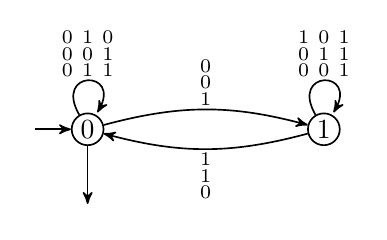
\begin{tikzpicture}[initial text=,->,>=stealth',semithick,auto,inner sep=1.2pt]
\tikzstyle{every state}=[minimum size=0.4]
\node[state,initial] (q0) at (0,0) {$0$};
  \node[state] (q1) at (3,0) {$1$};
   \node (q00-out) at (0,-1) {} ;
 \path (q0) edge node {} (q00-out);
\path (q0) edge[out=120,in=60,loop] node {$
  \begin{smallmatrix} 0 \\ 0 \\ 0 \end{smallmatrix}
  \begin{smallmatrix} 1 \\ 0  \\ 1 \end{smallmatrix}
  \begin{smallmatrix} 0 \\ 1 \\ 1 \end{smallmatrix}
$} (q0);
\path (q0) edge[bend left=15] node {$
  \begin{smallmatrix} 0 \\ 0 \\ 1 \end{smallmatrix}
$} (q1);
\path (q1) edge[out=120,in=60,loop] node {$
  \begin{smallmatrix}  1 \\ 0  \\ 0\end{smallmatrix}
  \begin{smallmatrix}  0 \\ 1 \\0 \end{smallmatrix}
  \begin{smallmatrix} 1 \\ 1 \\ 1 \end{smallmatrix}
$} (q1);
\path (q1) edge[bend left=15] node {$
  \begin{smallmatrix} 1 \\ 1 \\ 0 \end{smallmatrix}
$} (q0);
\end{tikzpicture}

\end{document}